\documentclass[
11pt, % The default document font size, options: 10pt, 11pt, 12pt
%codirector, % Uncomment to add a codirector to the title page
]{charter} 


% El títulos de la memoria, se usa en la carátula y se puede usar el cualquier lugar del documento con el comando \ttitle
\titulo{Detección y prevención de acciones maliciosas en agentes de inteligencia artificial} 

% Nombre del posgrado, se usa en la carátula y se puede usar el cualquier lugar del documento con el comando \degreename
%\posgrado{Carrera de Especialización en Sistemas Embebidos} 
%\posgrado{Carrera de Especialización en Internet de las Cosas} 
%\posgrado{Carrera de Especialización en Inteligencia Artificial}
%\posgrado{Maestría en Sistemas Embebidos} 
\posgrado{Maestría en Inteligencia Artificial}

% Tu nombre, se puede usar el cualquier lugar del documento con el comando \authorname
% IMPORTANTE: no omitir titulaciones ni tildación en los nombres, también se recomienda escribir los nombres completos (tal cual los tienen en su documento)
\autor{Esp. Ing. Florencia Priscilla Vela}

% El nombre del director y co-director, se puede usar el cualquier lugar del documento con el comando \supname y \cosupname y \pertesupname y \pertecosupname
\director{Ms. Abraham Adolfo Rodriguez Zepeda}
\pertenenciaDirector{FIUBA} 
\codirector{} % para que aparezca en la portada se debe descomentar la opción codirector en los parámetros de documentclass
\pertenenciaCoDirector{FIUBA}

% Nombre del cliente, quien va a aprobar los resultados del proyecto, se puede usar con el comando \clientename y \empclientename
\cliente{Nombre del cliente}
\empresaCliente{Empresa del cliente}
 
\fechaINICIO{19 de octubre de 2026}		%Fecha de inicio de la cursada de GdP \fechaInicioName
\fechaFINALPlan{7 de diciembre de 2026} 	%Fecha de final de cursada de GdP
\fechaFINALTrabajo{noviembre de 2027}	%Fecha de defensa pública del trabajo final


\begin{document}

\maketitle
\thispagestyle{empty}
\pagebreak


\thispagestyle{empty}
{\setlength{\parskip}{0pt}
\tableofcontents{}
}
\pagebreak


\section*{Registros de cambios}
\label{sec:registro}


\begin{table}[ht]
\label{tab:registro}
\centering
\begin{tabularx}{\linewidth}{@{}|c|X|c|@{}}
\hline
\rowcolor[HTML]{C0C0C0} 
Revisión & \multicolumn{1}{c|}{\cellcolor[HTML]{C0C0C0}Detalles de los cambios realizados} & Fecha      \\ \hline
0      & Creación del documento                                 &\fechaInicioName \\ \hline
1      & Se completa hasta el punto 6 inclusive                & 29 de octubre de 2026 \\ \hline
2      & Se realizan las correcciones recomendadas y se completa hasta el punto 9 inclusive & 6 de noviembre de 2026 \\ \hline
%3      & Se completa hasta el punto 12 inclusive                & {día} de {mes} de 202X \\ \hline
%4      & Se completa el plan	                                 & {día} de {mes} de 202X \\ \hline

% Si hay más correcciones pasada la versión 4 también se deben especificar acá

\end{tabularx}
\end{table}

\pagebreak



\section*{Acta de constitución del proyecto}
\label{sec:acta}

\begin{flushright}
Buenos Aires, \fechaInicioName
\end{flushright}

\vspace{2cm}

Por medio de la presente se acuerda con el \authorname\hspace{1px} que su Trabajo Final de la \degreename\hspace{1px} se titulará ``\ttitle'' y consistirá en el desarrollo de un sistema que evalúa cada acción propuesta por un agente de IA antes de ejecutarla y decide si permitirla, revisarla o bloquearla según su riesgo. El trabajo tendrá un presupuesto preliminar estimado de 600 horas y un costo estimado de USD~9.490, con fecha de inicio el \fechaInicioName\hspace{1px} y fecha de presentación pública en \fechaFinalName.

Se adjunta a esta acta la planificación inicial.

\vfill

% Esta parte se construye sola con la información que hayan cargado en el preámbulo del documento y no debe modificarla
\begin{table}[ht]
\centering
\begin{tabular}{c}
\begin{tabular}[c]{@{}c@{}}Dr. Ing. Ariel Lutenberg \\ Director posgrado FIUBA\end{tabular} \vspace{2.5cm} \\
\begin{tabular}[c]{@{}c@{}} \supname \\ Director del Trabajo Final\end{tabular} \vspace{2.5cm} \\
\end{tabular}
\end{table}

\pagebreak

\section{1. Descripción técnica-conceptual del proyecto a realizar}
\label{sec:descripcion}

\subsection{Contexto y motivación}

Los modelos de lenguaje de gran escala (en inglés, \textit{Large Language Models} o LLM) se difundieron como sistemas conversacionales capaces de procesar y generar texto. A partir de estas capacidades se desarrollaron los agentes de inteligencia artificial (IA), que incorporan la capacidad de planificar y ejecutar tareas mediante herramientas. Así, además de responder consultas, un agente puede leer y modificar archivos, ejecutar comandos, enviar correos o utilizar servicios externos. Esta capacidad de acción amplía sus posibilidades de aplicación, pero también les permite acceder a recursos sensibles y genera nuevos riesgos de seguridad.

Uno de estos riesgos se presenta cuando un agente consulta una página web o un documento que contiene instrucciones maliciosas. El agente puede interpretar esas instrucciones como parte de la solicitud original y actuar en consecuencia. Este tipo de ataque, conocido como \textit{prompt injection} o inyección de instrucciones, podría llevarlo a divulgar información sensible, enviar datos a destinos no autorizados, modificar o borrar recursos sin permiso, ejecutar código no aprobado o intentar ampliar sus privilegios. El momento de la detección es fundamental, ya que, si el desvío se identifica después de ejecutar la acción, el daño puede ser difícil o imposible de revertir. Por eso, resulta necesario contar con controles que evalúen las acciones antes de que se ejecuten.

\subsection{Descripción funcional y técnica}

En este contexto, el proyecto propone desarrollar un componente de control que actúe como intermediario entre el agente y sus herramientas. Su función es evaluar cada acción propuesta y decidir si corresponde permitirla, enviarla a revisión o bloquearla antes de su ejecución. Se trata de una iniciativa académica individual en el marco del Trabajo Final de la Maestría en Inteligencia Artificial. El proyecto está dirigido a personas u organizaciones que utilizan agentes para trabajar con datos, archivos o servicios y necesitan delegar tareas sin exponer recursos sensibles. Para estos usuarios, resultan especialmente relevantes la preservación de la privacidad y la precisión de las alertas, de manera que el sistema detecte acciones riesgosas sin interrumpir innecesariamente las tareas legítimas.

Para tomar cada decisión, el sistema considera tres fuentes de información: los permisos del agente, la herramienta que pretende utilizar junto con sus argumentos y el contexto reciente de la sesión. La evaluación combina el grado en que una acción se aparta del comportamiento esperado con su coherencia respecto del objetivo de la tarea y los permisos otorgados. Se busca que el control funcione en tiempo real, con baja latencia, y que pueda ejecutarse de manera local y liviana en la máquina del usuario para preservar la privacidad.

El funcionamiento del componente de control se presenta en la figura~\ref{fig:diagBloques}. Cuando el agente propone una acción, el componente de control aplica primero un conjunto de reglas explícitas de permisos independientes del modelo de IA. Por ejemplo, una regla puede impedir que un agente con determinado rol lea un archivo de credenciales. Si estas reglas no son suficientes para resolver la decisión, interviene un modelo de riesgo que evalúa la acción considerando el contexto de la sesión. La decisión final integra ambos mecanismos: solo las acciones clasificadas como permitidas llegan al ejecutor; las que requieren revisión quedan pendientes y las bloqueadas no se ejecutan. Las restricciones establecidas por las reglas mantienen su validez independientemente de la puntuación del modelo, de modo que este no puede anular una prohibición explícita.

\begin{figure}[H]
\centering
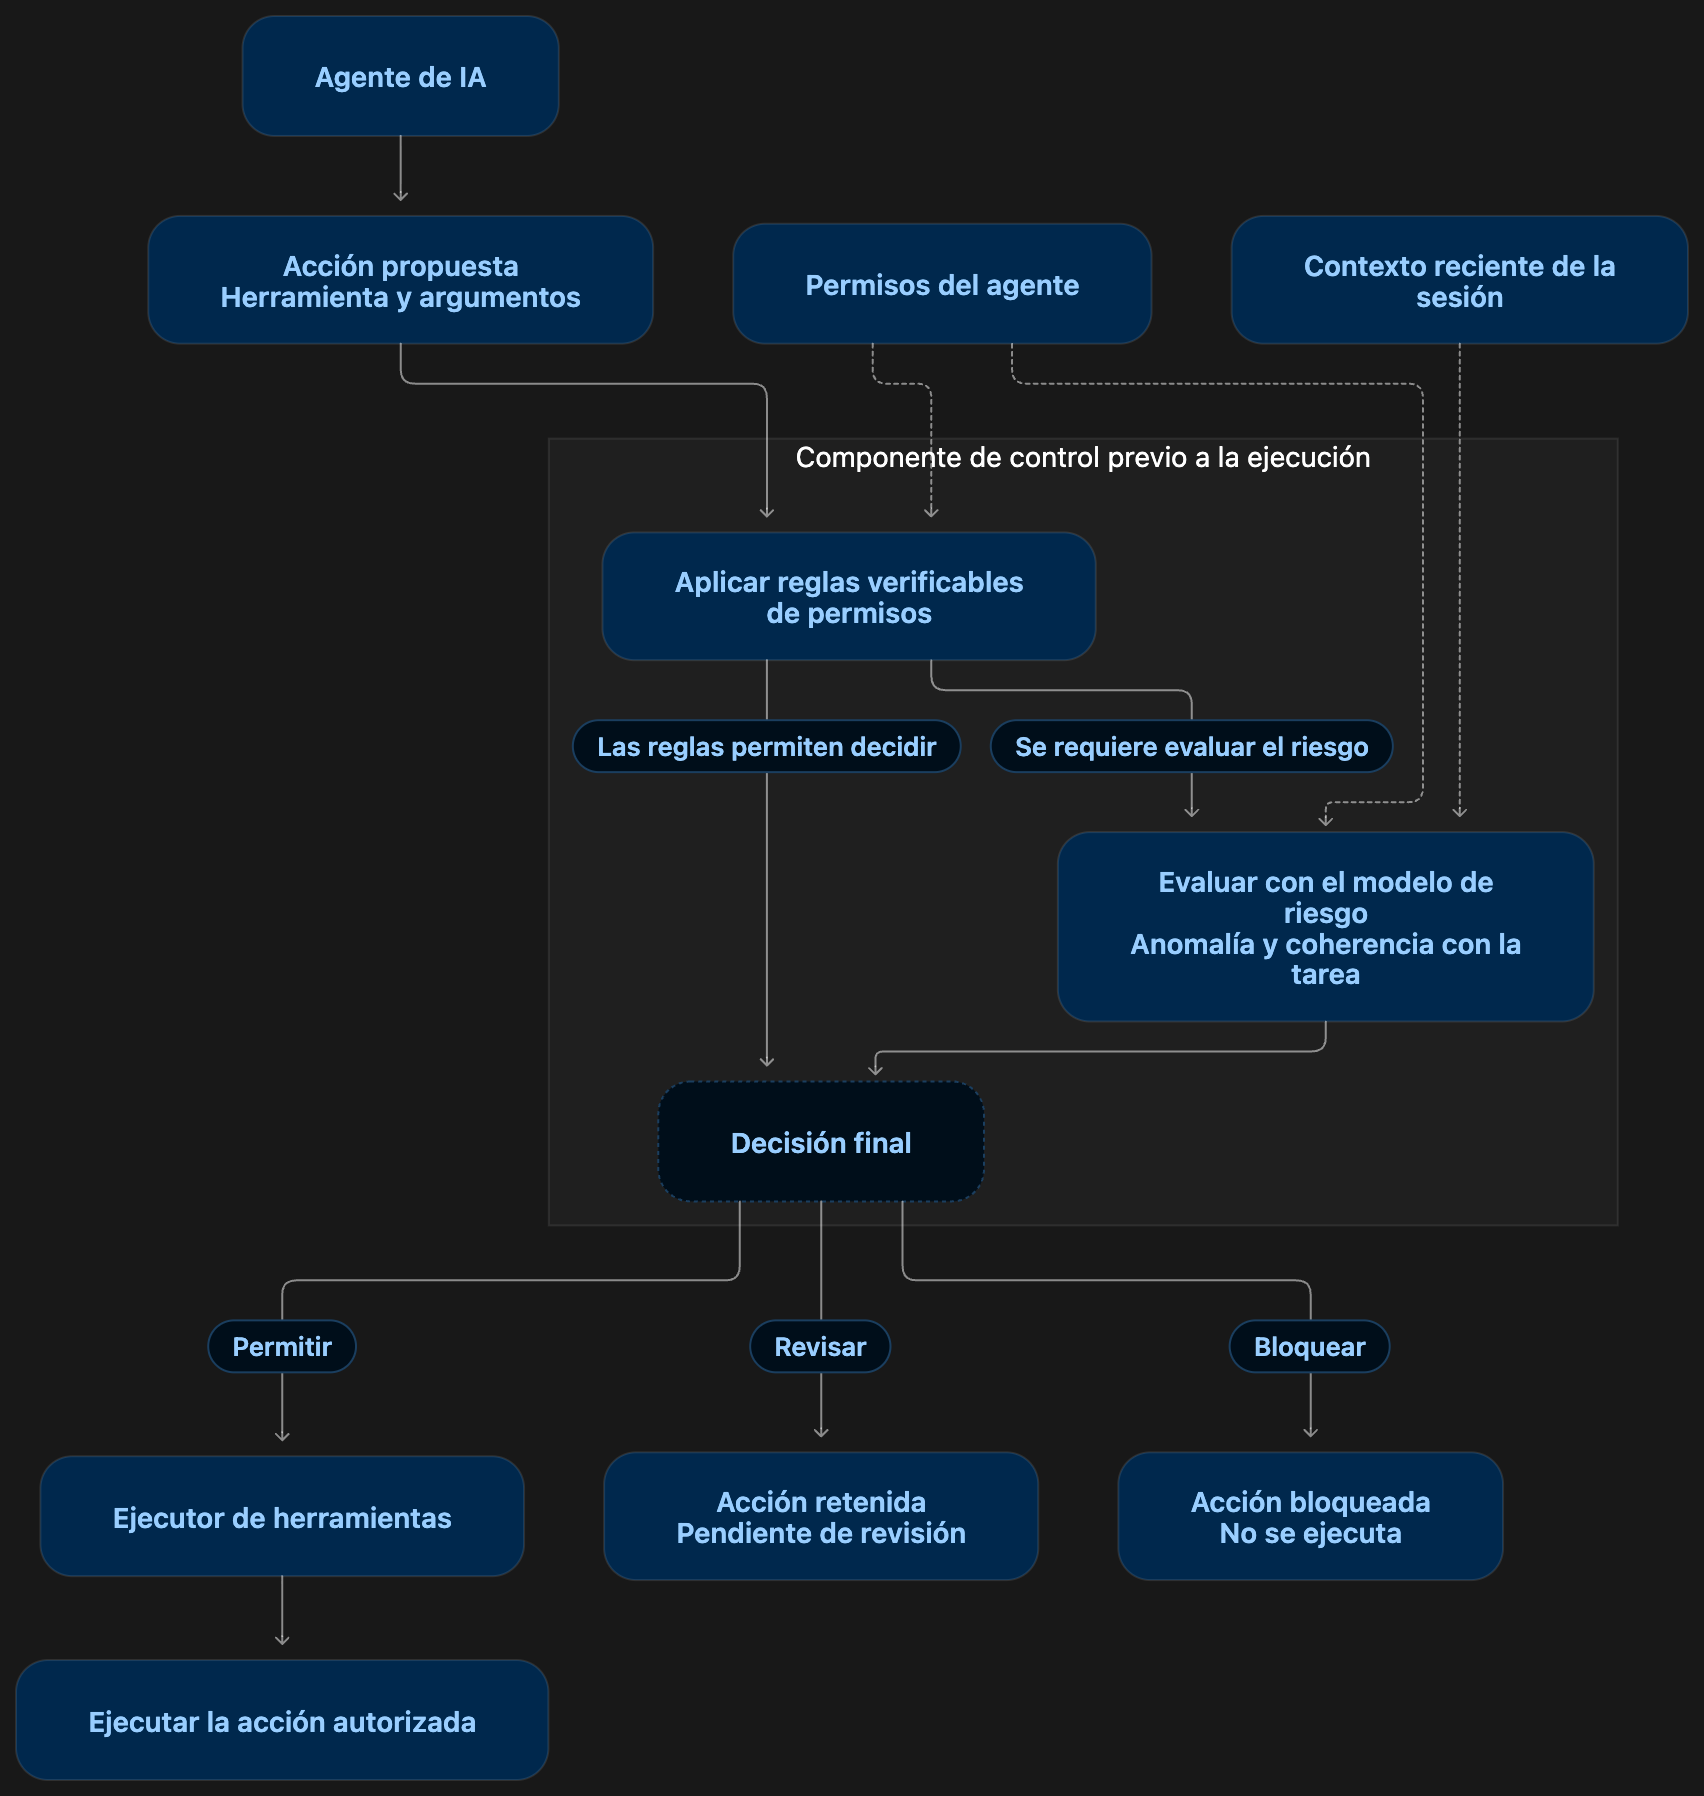
\includegraphics[width=0.85\textwidth]{./Figuras/diagBloques.png}
\caption{Diagrama en bloques del sistema.}
\label{fig:diagBloques}
\end{figure}

\subsection{Estado del arte}

En cuanto al estado del arte, se identifican distintas líneas de trabajo relacionadas con el problema. Una de ellas comprende modelos de protección como Llama Guard, ShieldGemma y Granite Guardian, que permiten detectar riesgos en las entradas y respuestas de los modelos de lenguaje. Otra incluye modelos orientados a producir decisiones estructuradas a partir de un contexto y una pregunta, como Jev y Laya. Estos modelos pueden devolver una categoría, una puntuación o una probabilidad, por lo que constituyen alternativas para explorar en la evaluación de acciones. También existen mecanismos de control sobre el uso de herramientas, como Invariant Guardrails y Progent, y sistemas de protección para agentes, como LlamaFirewall. A estas líneas se suman las técnicas de detección de anomalías de comportamiento, que permiten identificar desviaciones respecto de patrones habituales.

\subsection{Grado de innovación}

La principal innovación del proyecto está en controlar cada acción en el instante previo a su ejecución, antes de que un desvío pueda provocar un daño difícil de revertir, en lugar de detectarlo una vez producido. A su vez, las reglas de permisos verificables operan con prioridad sobre el modelo de riesgo, de manera que una prohibición explícita nunca puede ser anulada por su puntuación.

Además, se busca que el sistema pueda ejecutarse en equipos con recursos computacionales limitados. Para ello se explorarán variantes cuantizadas, que reducen los requisitos de memoria y facilitan el uso de modelos en máquinas de capacidad limitada. La propuesta combina reglas verificables con una evaluación contextual del riesgo, y su utilidad deberá analizarse en comparación con los enfoques existentes, considerando tanto la detección de acciones riesgosas como la latencia y el consumo de recursos.

\subsection{Conjunto de datos y estrategia de experimentación}

Una de las etapas más importantes será definir el conjunto de datos sobre el cual se realizarán las pruebas, ya que caracterizar un comportamiento como malicioso constituye un problema complejo. Una misma acción puede ser legítima o riesgosa según el objetivo de la tarea, los permisos otorgados, los recursos involucrados y el contexto en el que se propone. Además, una acción poco habitual no necesariamente es maliciosa, y una acción frecuente puede resultar perjudicial si se realiza sin autorización.

Por este motivo, la construcción del conjunto de datos requerirá establecer criterios claros para distinguir acciones permitidas, acciones que requieren revisión y acciones que deben bloquearse. Se prevé considerar datos públicos y ejemplos sintéticos que representen tanto tareas legítimas como intentos de desvío y situaciones ambiguas. Sobre esta base se compararán detectores de anomalías, clasificadores supervisados y modelos de decisión preentrenados, con el objetivo de identificar qué enfoques ofrecen el equilibrio más adecuado entre detección de riesgos, precisión de las alertas y requisitos de ejecución.

\section{2. Identificación y análisis de los interesados}
\label{sec:interesados}

En la tabla~\ref{tab:interesados} se identifican los interesados del proyecto. Al tratarse de un Trabajo Final de carácter académico e individual, varios roles habituales en proyectos mayores (auspiciante, impulsor, colaboradores, equipo, opositores) no aplican y se omiten.

\begin{table}[ht]
\caption{Identificación de los interesados.}
\label{tab:interesados}
\begin{tabularx}{\linewidth}{@{}|l|X|l|X|@{}}
\hline
\rowcolor[HTML]{C0C0C0}
Rol           & Nombre y Apellido & Organización 	& Puesto 	\\ \hline
Responsable   & \authorname       & FIUBA        	& Alumna 	\\ \hline
Orientador    & \supname	      & \pertesupname 	& Director del Trabajo Final \\ \hline
Usuario final & Personas y equipos técnicos que utilizan agentes de IA & - & Desarrolladores, analistas y perfiles de finanzas, RR.\,HH.\ e IT \\ \hline
\end{tabularx}
\end{table}

A continuación se describen las principales características de cada interesado:
\begin{itemize}
	\item \textbf{Responsable:} ejecuta la totalidad del trabajo técnico y la redacción de la memoria. Su disponibilidad es de tipo \textit{part-time}, lo que condiciona el cronograma y obliga a planificar con holgura.
	\item \textbf{Orientador:} el Director del Trabajo Final es experto en la temática y colabora en la definición de los requerimientos, la metodología de evaluación y la revisión de la memoria.
	\item \textbf{Usuario final:} valora la privacidad (que sus datos no salgan de su equipo), un bajo impacto en la fluidez de uso (pocas falsas alarmas) y que la solución funcione en computadoras de capacidad modesta.
\end{itemize}


\section{3. Propósito del proyecto}
\label{sec:proposito}

Evaluar y construir un sistema capaz de detectar, evaluar y controlar acciones maliciosas de agentes de inteligencia artificial antes de su ejecución. Se prioriza una ejecución liviana y local para preservar la privacidad del usuario siempre que sea posible, sin descartar otras alternativas, como el uso de la nube, según las capacidades del equipo. También se propone entregar evidencia reproducible sobre qué enfoques ofrecen el mejor equilibrio entre seguridad (detectar ataques), usabilidad (pocas falsas alarmas) y costo computacional (latencia, memoria y tamaño). Estos enfoques incluyen la detección de anomalías, los clasificadores entrenados, los modelos de decisión preentrenados y sus combinaciones. Además, se contemplarán versiones adaptadas a distintos niveles de recursos del equipo del usuario.

\section{4. Alcance del proyecto}
\label{sec:alcance}

El proyecto incluye:
\begin{itemize}
	\item Revisión del estado del arte y preparación de los datos: conjuntos públicos disponibles y de un conjunto sintético propio.
	\item Implementación de tres familias de detectores y de su combinación:
		\begin{itemize}
		\item detección de anomalías: identifica lo que se aparta de lo normal sin requerir ejemplos de ataques
		\item clasificadores entrenados: aprenden de ejemplos etiquetados a distinguir una acción riesgosa de una legítima
		\item modelos de decisión preentrenados: modelos pequeños y rápidos que eligen entre opciones.
		\end{itemize}
	\item Un banco de pruebas (\textit{benchmark}) reproducible que mida, para cada enfoque: cuántos ataques detecta antes de ejecutarse, cuántas falsas alarmas genera (por acción y por sesión), la latencia, la memoria RAM, el tamaño del modelo y el uso de cómputo.
	\item Técnicas de optimización: cuantización (compresión) y comparación de versiones del mismo modelo en distintas precisiones, para hacerlo viable en equipos modestos.
	\item Un intermediario configurable (el \textit{gate}) que se interpone entre el agente y sus herramientas, con una matriz de decisión que elige la mejor variante según el entorno (nube autorizada, GPU local, o poca memoria RAM, caso en el que se usa la versión liviana).
	\item La memoria del Trabajo Final, el código fuente documentado y los resultados reproducibles.
\end{itemize}

El proyecto no incluye:
\begin{itemize}
	\item Un producto comercial listo para producción.
	\item El entrenamiento de modelos de lenguaje grandes desde cero; se parte de modelos existentes.
	\item La integración con un \textit{sandbox} de agentes; esto quedaría como trabajo futuro o prueba exploratoria.
	\item La recolección de datos reales de usuarios; se trabaja con datos públicos y sintéticos, por lo que los resultados no se reportan como incidentes reales confirmados.
\end{itemize}


\section{5. Supuestos del proyecto}
\label{sec:supuestos}

Para el desarrollo del proyecto se supone que:
\begin{itemize}
	\item Se dispone de conjuntos de datos públicos que pueden utilizarse como referencia para estudiar y evaluar técnicas de detección de comportamientos riesgosos en agentes de inteligencia artificial.
	\item Se dispone de acceso a modelos abiertos en repositorios como Hugging Face y GitHub.
	\item Se cuenta con acceso a cómputo con GPU de forma gratuita o de bajo costo (por ejemplo, Google Colab) para las partes que lo requieran; el resto corre en una computadora personal.
	\item La disponibilidad horaria de la responsable permite sostener las 600~h estimadas, distribuidas en el período de ejecución (modalidad \textit{part-time}), con la orientación periódica del director.
	\item Las licencias de los modelos y conjuntos de datos de terceros permiten su uso con fines académicos y de investigación.
	\item La disponibilidad de los servicios de cómputo y el acceso a internet se mantienen razonablemente estables durante el proyecto.
	\item Los resultados se evalúan sobre datos sintéticos o de laboratorio; se asume que esto es suficiente para comparar enfoques entre sí, aunque no para afirmar su eficacia en un entorno de producción real.
\end{itemize}

\section{6. Requerimientos}
\label{sec:requerimientos}

Los requerimientos se agrupan por afinidad.

\begin{enumerate}
	\item Requerimientos funcionales:
		\begin{enumerate}
			\item El sistema debe evaluar cada acción propuesta por el agente antes de ejecutarla y emitir una de tres decisiones: permitir, revisar o bloquear.
			\item El sistema debe usar como entrada únicamente información disponible antes de la acción (contexto de la sesión, herramienta, argumentos y permisos). No debe utilizar información posterior a la acción ni las etiquetas de referencia empleadas durante el entrenamiento o la evaluación.
			\item El sistema debe aplicar reglas de permisos verificables, independientes del modelo de IA (por ejemplo, denegar la lectura de archivos de credenciales).
			\item El sistema debe permitir intercambiar el mecanismo de evaluación del riesgo (detección de anomalías, clasificación o modelo preentrenado) sin modificar el resto de los componentes.
			\item El sistema debe soportar perfiles por usuario y por grupo de actividad, e identificar desviaciones respecto de los patrones de comportamiento habituales.
			\item El componente debe seleccionar automáticamente la variante del modelo de evaluación de riesgo en función de los recursos computacionales disponibles en el entorno de ejecución, que considere la capacidad de CPU, la disponibilidad de GPU y la posibilidad de utilizar servicios en la nube.
		\end{enumerate}
	\item Requerimientos de desempeño:
		\begin{enumerate}
			\item El sistema debe tomar cada decisión rápidamente; en la variante liviana ejecutada en CPU, el tiempo promedio entre la recepción de una solicitud y la emisión de una decisión no debe superar los 500~ms.
			\item El sistema debe poder funcionar usando como mucho 2~GB de memoria RAM adicional.
			\item El sistema debe ocupar como máximo 1~GB en disco.
		\end{enumerate}
	\item Requerimientos de seguridad y privacidad:
		\begin{enumerate}
			\item El sistema debe ofrecer un modo de funcionamiento en el que toda la inferencia se ejecute localmente, sin transmitir datos a servicios externos.
			\item El uso de la nube debe ser opcional y explícitamente autorizado por el usuario.
		\end{enumerate}
	\item Requerimientos de documentación:
		\begin{enumerate}
			\item Memoria del Trabajo Final.
			\item Documentación que permita reproducir los experimentos con los conjuntos de datos públicos.
			\item Documentación de los conjuntos de datos, con su origen y sus códigos de verificación de integridad (en inglés, \textit{checksums}).
		\end{enumerate}
	\item Requerimientos de testing:
		\begin{enumerate}
			\item El proyecto debe incluir pruebas automatizadas del componente de control que verifiquen las decisiones de permitir, revisar y bloquear acciones, así como el cumplimiento de las reglas de permisos.
		\end{enumerate}
	\item Requerimientos de interoperabilidad:
		\begin{enumerate}
			\item El sistema debe exponer su evaluación mediante una función que reciba el contexto de la sesión y la acción propuesta y devuelva la decisión: permitir, revisar o bloquear. La interfaz debe ser independiente del modelo de riesgo utilizado internamente, de modo que este pueda cambiarse sin alterar la forma de invocación.
		\end{enumerate}
	\item Requerimientos regulatorios y de normas:
		\begin{enumerate}
			\item Cumplir con la normativa de protección de datos personales aplicable (en Argentina, la Ley 25.326; se consideran además principios del GDPR por buenas prácticas), dado que el sistema observa el comportamiento de los usuarios: minimización de datos, procesamiento local y anonimización cuando corresponda.
			\item Respetar las licencias de los conjuntos de datos y modelos de terceros.
		\end{enumerate}
\end{enumerate}

\section{7. Historias de usuarios (\textit{Product backlog})}
\label{sec:backlog}

Las historias de usuario se derivan de los requerimientos (sección~\ref{sec:requerimientos}) y del alcance (sección~\ref{sec:alcance}). Se escriben desde la perspectiva de quienes desean cada capacidad: el usuario final (personas y equipos que delegan tareas en agentes de IA), el administrador de seguridad (quien configura reglas y perfiles), el desarrollador integrador (quien incorpora el \textit{gate} a una plataforma anfitriona) y la responsable del Trabajo Final (en su rol de investigadora y de desarrolladora de la solución).

\textbf{Criterio de ponderación.} El tamaño de cada historia se expresa en \textit{story points} y se calcula como la suma de tres factores, cada uno valorado en una escala de 1 a 5:
\begin{itemize}
	\item \textbf{Complejidad:} cantidad de componentes del sistema involucrados y su grado de interacción.
	\item \textbf{Dificultad:} esfuerzo técnico y conocimiento necesarios para implementar la historia.
	\item \textbf{Incertidumbre:} desconocimiento inicial o riesgo de que los supuestos cambien durante el desarrollo.
\end{itemize}
De este modo, el puntaje mínimo posible es 3 y el máximo 15. Cuanto mayor es el valor, mayor es el tamaño relativo de la historia.

\begin{enumerate}
	\item Como usuario final que delega tareas en un agente de IA, \\
	quiero que cada acción propuesta se evalúe antes de ejecutarse y se clasifique en permitir, revisar o bloquear, \\
	para evitar que una acción riesgosa provoque un daño difícil de revertir.

	\textit{Story points}: 12 (complejidad: 5, dificultad: 4, incertidumbre: 3) \\
	\textit{Prioridad}: alta

	\item Como usuario final, \\
	quiero que la decisión se tome usando únicamente información disponible antes de la acción (contexto de la sesión, herramienta, argumentos y permisos), \\
	para asegurar que el sistema utiliza únicamente información disponible en el momento de tomar la decisión.

	\textit{Story points}: 8 (complejidad: 2, dificultad: 3, incertidumbre: 3) \\
	\textit{Prioridad}: alta

	\item Como administrador de seguridad, \\
	quiero definir reglas de permisos verificables e independientes del modelo de IA (por ejemplo, prohibir la lectura de archivos de credenciales), \\
	para garantizar prohibiciones que el modelo no pueda anular.

	\textit{Story points}: 6 (complejidad: 2, dificultad: 2, incertidumbre: 2) \\
	\textit{Prioridad}: alta

	\item Como investigadora, \\
	quiero poder intercambiar el mecanismo de evaluación del riesgo (anomalías, clasificador o decisión preentrenada) sin modificar el resto del sistema, \\
	para comparar los distintos enfoques en igualdad de condiciones.

	\textit{Story points}: 8 (complejidad: 3, dificultad: 3, incertidumbre: 2) \\
	\textit{Prioridad}: alta

	\item Como administrador de seguridad, \\
	quiero perfiles por usuario y por grupo de actividad que permitan identificar desviaciones respecto del patrón habitual, \\
	para detectar comportamientos anómalos según el contexto de cada rol.

	\textit{Story points}: 11 (complejidad: 3, dificultad: 4, incertidumbre: 4) \\
	\textit{Prioridad}: media

	\item Como usuario final con un equipo de recursos computacionales limitados, \\
	quiero que el sistema elija automáticamente la variante de modelo según los recursos del entorno (nube, GPU o CPU con poca memoria RAM), \\
	para usar la solución sin tener que configurarla manualmente.

	\textit{Story points}: 8 (complejidad: 3, dificultad: 3, incertidumbre: 2) \\
	\textit{Prioridad}: media

	\item Como usuario final, \\
	quiero que el sistema emita cada decisión en un tiempo promedio no superior a 500~ms cuando se ejecute la variante liviana sobre CPU, \\
	para no entorpecer el flujo de trabajo del agente.

	\textit{Story points}: 10 (complejidad: 2, dificultad: 4, incertidumbre: 4) \\
	\textit{Prioridad}: media

	\item Como usuario final, \\
	quiero que la inferencia se ejecute de forma 100\,\% local sin enviar datos a internet, y que el uso de la nube sea opcional y explícitamente autorizado, \\
	para preservar la privacidad de mi información.

	\textit{Story points}: 6 (complejidad: 2, dificultad: 2, incertidumbre: 2) \\
	\textit{Prioridad}: media

	\item Como desarrollador integrador, \\
	quiero una función que reciba el contexto de la sesión y la acción propuesta y devuelva la decisión, \\
	para incorporar el \textit{gate} al entorno que ejecuta al agente sin acoplarlo a una implementación particular.

	\textit{Story points}: 5 (complejidad: 2, dificultad: 2, incertidumbre: 1) \\
	\textit{Prioridad}: alta

	\item Como investigadora, \\
	quiero un banco de pruebas (\textit{benchmark}) reproducible que mida, por enfoque, la tasa de detección de ataque, las falsas alarmas, la latencia, la memoria RAM, el tamaño del modelo y el uso de cómputo, \\
	para identificar el mejor equilibrio entre seguridad, usabilidad y costo.

	\textit{Story points}: 10 (complejidad: 4, dificultad: 3, incertidumbre: 3) \\
	\textit{Prioridad}: media

	\item Como investigadora, \\
	quiero construir un conjunto de datos con ejemplos públicos y sintéticos y criterios claros de permitir, revisar o bloquear, \\
	para entrenar y evaluar los detectores sobre tareas legítimas, intentos de desvío y situaciones ambiguas.

	\textit{Story points}: 13 (complejidad: 4, dificultad: 4, incertidumbre: 5) \\
	\textit{Prioridad}: alta

	\item Como investigadora, \\
	quiero aplicar cuantización y comparar versiones del mismo modelo en distintas precisiones, \\
	para hacerlo viable en equipos modestos sin perder demasiada capacidad de detección.

	\textit{Story points}: 9 (complejidad: 3, dificultad: 3, incertidumbre: 3) \\
	\textit{Prioridad}: baja

	\item Como responsable del proyecto, \\
	quiero pruebas automatizadas del \textit{gate}, \\
	para asegurar que las reglas y las decisiones se mantienen correctas frente a los cambios del sistema.

	\textit{Story points}: 5 (complejidad: 2, dificultad: 2, incertidumbre: 1) \\
	\textit{Prioridad}: baja
\end{enumerate}

El total acumulado del \textit{product backlog} es de 111 \textit{story points}.

\pagebreak

\section{8. Entregables principales del proyecto}
\label{sec:entregables}

Los entregables principales del proyecto son:

\begin{itemize}
	\item Memoria del Trabajo Final.
	\item Código fuente documentado del componente de control (el \textit{gate}), el motor de reglas de permisos verificables y los detectores de riesgo.
	\item Implementación de las tres familias de detectores (anomalías, clasificadores entrenados y modelos de decisión preentrenados) y de su combinación.
	\item Conjunto de datos de evaluación, con datos públicos curados y ejemplos sintéticos, junto con su documentación, origen y códigos de verificación de integridad (en inglés, \textit{checksums}).
	\item Banco de pruebas (\textit{benchmark}) reproducible, con las métricas de detección, falsas alarmas, latencia, memoria, tamaño del modelo y uso de cómputo.
	\item Resultados experimentales reproducibles, con las tablas y figuras comparativas de los distintos enfoques.
	\item Documentación que permita reproducir los experimentos, con las instrucciones de instalación y ejecución.
\end{itemize}

\section{9. Desglose del trabajo en tareas}
\label{sec:wbs}

Las tareas se agrupan por afinidad y se relacionan con los requerimientos definidos en la sección~\ref{sec:requerimientos}. La estimación se expresa en horas (h).

\begin{enumerate}
\item Gestión y organización del proyecto (38 h)
	\begin{enumerate}
	\item Planificación del proyecto y elaboración del plan de GdP (24 h)
	\item Seguimiento del avance y reuniones de orientación con el director (14 h)
	\end{enumerate}
\item Relevamiento y estado del arte (56 h)
	\begin{enumerate}
	\item Revisión de la literatura sobre \textit{prompt injection} y seguridad en agentes (20 h)
	\item Estudio de modelos de protección existentes (Llama Guard, ShieldGemma, Granite Guardian, entre otros) (20 h)
	\item Estudio de mecanismos de control de herramientas y de detección de anomalías (16 h)
	\end{enumerate}
\item Conjunto de datos (84 h)
	\begin{enumerate}
	\item Definición de criterios para distinguir acciones permitidas, a revisar y a bloquear (20 h)
	\item Recopilación y curación de conjuntos de datos públicos (24 h)
	\item Generación de ejemplos sintéticos (tareas legítimas, intentos de desvío y casos ambiguos) (24 h)
	\item Documentación del conjunto de datos y cálculo de \textit{checksums} (16 h)
	\end{enumerate}
\item Desarrollo de los detectores (122 h)
	\begin{enumerate}
	\item Implementación del detector por anomalías (30 h)
	\item Implementación de los clasificadores entrenados (30 h)
	\item Integración de los modelos de decisión preentrenados (32 h)
	\item Combinación de los detectores (30 h)
	\end{enumerate}
\item Optimización y cuantización (46 h)
	\begin{enumerate}
	\item Cuantización de los modelos (22 h)
	\item Comparación de versiones en distintas precisiones y su costo (24 h)
	\end{enumerate}
\item Intermediario (\textit{gate}) e integración (66 h)
	\begin{enumerate}
	\item Diseño e implementación del motor de reglas de permisos verificables (24 h)
	\item Implementación del \textit{gate} y de su interfaz (contexto y acción a decisión) (22 h)
	\item Matriz de decisión y selección automática de la variante según los recursos (20 h)
	\end{enumerate}
\item Evaluación y banco de pruebas (66 h)
	\begin{enumerate}
	\item Diseño del \textit{benchmark} y de las métricas (20 h)
	\item Ejecución de los experimentos (26 h)
	\item Análisis de los resultados (20 h)
	\end{enumerate}
\item Pruebas automatizadas (18 h)
	\begin{enumerate}
	\item Desarrollo de las pruebas automatizadas del \textit{gate} (18 h)
	\end{enumerate}
\item Memoria del Trabajo Final (46 h)
	\begin{enumerate}
	\item Redacción de la memoria (26 h)
	\item Revisión e incorporación de correcciones (20 h)
	\end{enumerate}
\item Presentación y cierre (18 h)
	\begin{enumerate}
	\item Elaboración de la presentación (10 h)
	\item Ensayo de la presentación y cierre del proyecto (8 h)
	\end{enumerate}
\item Buffer para imprevistos (40 h)
	\begin{enumerate}
	\item Tiempo reservado para retrasos, cambios de alcance y problemas técnicos (40 h)
	\end{enumerate}
\end{enumerate}

Cantidad total de horas: 600 h.

\section{10. Diagrama de Activity On Node}
\label{sec:AoN}

\begin{consigna}{red}
Armar el AoN a partir del WBS definido en la etapa anterior.

Una herramienta simple para desarrollar los diagramas es el Draw.io (\url{https://app.diagrams.net/}).
\href{https://app.diagrams.net}{Draw.io}


\begin{figure}[htpb]
\centering 
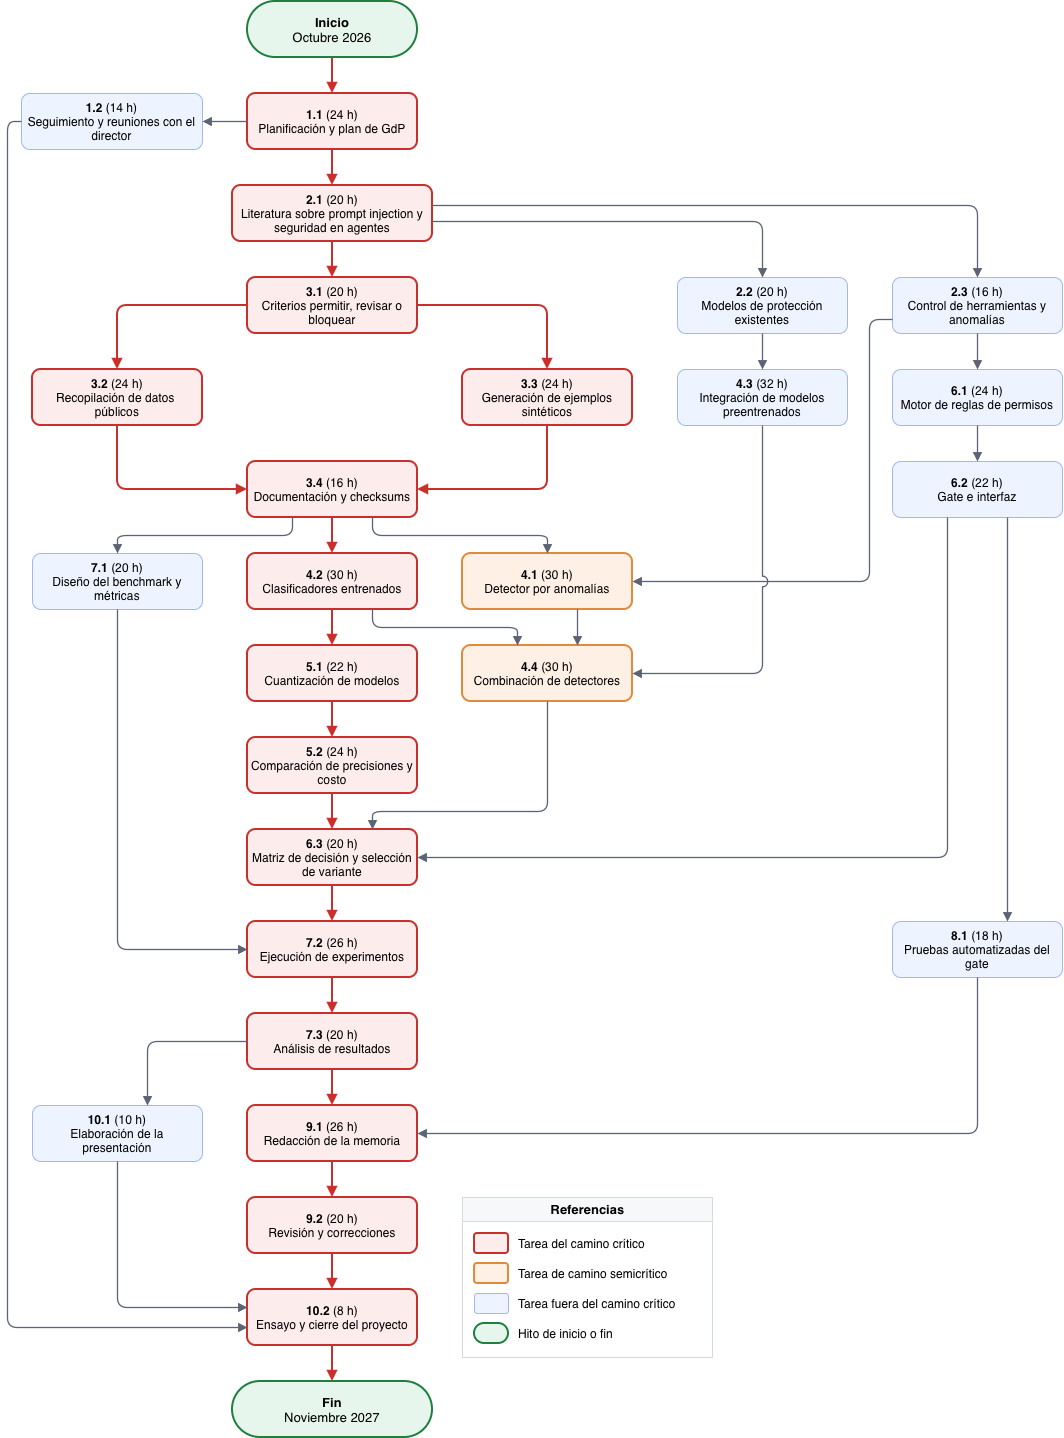
\includegraphics[width=.8\textwidth]{./Figuras/AoN.png}
\caption{Diagrama de \textit{Activity on Node}.}
\label{fig:AoN}
\end{figure}

Indicar claramente en qué unidades están expresados los tiempos.
De ser necesario indicar los caminos semi críticos y analizar sus tiempos mediante un cuadro.
Es recomendable usar colores y un cuadro indicativo describiendo qué representa cada color.

\end{consigna}

\section{11. Diagrama de Gantt}
\label{sec:gantt}

\begin{consigna}{red}
Existen muchos programas y recursos \textit{online} para hacer diagramas de Gantt, entre los cuales destacamos:

\begin{itemize}
\item Planner
\item GanttProject
\item Trello + \textit{plugins}. En el siguiente link hay un tutorial oficial: \\ \url{https://blog.trello.com/es/diagrama-de-gantt-de-un-proyecto}
\item Creately, herramienta online colaborativa. \\\url{https://creately.com/diagram/example/ieb3p3ml/LaTeX}
\item Se puede hacer en latex con el paquete \textit{pgfgantt}\\ \url{http://ctan.dcc.uchile.cl/graphics/pgf/contrib/pgfgantt/pgfgantt.pdf}
\end{itemize}

Pegar acá una captura de pantalla del diagrama de Gantt, cuidando que la letra sea suficientemente grande como para ser legible. 
Si el diagrama queda demasiado ancho, se puede pegar primero la ``tabla'' del Gantt y luego pegar la parte del diagrama de barras del diagrama de Gantt.

Configurar el software para que en la parte de la tabla muestre los códigos del EDT (WBS).\\
Configurar el software para que al lado de cada barra muestre el nombre de cada tarea.\\
Revisar que la fecha de finalización coincida con lo indicado en el Acta Constitutiva.

En la figura \ref{fig:gantt}, se muestra un ejemplo de diagrama de gantt realizado con el paquete de \textit{pgfgantt}. 
En la plantilla pueden ver el código que lo genera y usarlo de base para construir el propio.

Las fechas pueden ser calculadas utilizando alguna de las herramientas antes citadas. Sin embargo, el siguiente ejemplo
fue elaborado utilizando 
\href{https://docs.google.com/spreadsheets/d/1fBz8NhSpc4tkkhz3KjJCbh1nR_ltDkfEcZi4tZXduqs}{esta hoja de cálculo}.

Es importante destacar que el ancho del diagrama estará dado por la longitud del texto utilizado para las tareas 
(Ejemplo: tarea 1, tarea 2, etcétera) y el valor \textit{x unit}. Para mejorar la apariencia del diagrama, es necesario
ajustar este valor y, quizás, acortar los nombres de las tareas.

\begin{figure}[htpb]
  \begin{center}
    \begin{ganttchart}[
      time slot unit=day,
      time slot format=isodate,
      x unit=0.038cm,
      y unit title=0.7cm,
      y unit chart=0.6cm,
      milestone/.append style={xscale=4}
      ]{2021-03-05}{2021-12-16}
      \gantttitlecalendar*{2021-03-05}{2021-12-16}{year} \\
      \gantttitlecalendar*{2021-03-05}{2021-12-16}{month} \\
      \ganttgroup{Duración Total}{2021-03-05}{2021-12-16} \\
      %%%%%%%%%%%%%%%%%Organización
      \ganttgroup{Organización}{2021-03-05}{2021-04-16} \\
      \ganttbar{Planificación del proyecto}{2021-03-05}{2021-04-15} \\
      %%%%%%%%%%%%%%%%%Ejecución
      \ganttgroup{Ejecución}{2021-04-16}{2021-10-21} \\
      \ganttbar{Tarea 1}{2021-04-16}{2021-04-29} \\
      \ganttbar{Tarea 2}{2021-04-30}{2021-05-13} \\
      \ganttbar{Tarea 3}{2021-05-14}{2021-05-27} \\
      \ganttbar{Tarea 4}{2021-05-28}{2021-07-12} \\
      \ganttbar{Tarea 5}{2021-07-13}{2021-08-09} \\
      \ganttbar{Tarea 6}{2021-08-10}{2021-09-23} \\
      \ganttbar{Tarea 7}{2021-09-24}{2021-09-30} \\
      \ganttbar{Tarea 8}{2021-10-01}{2021-10-14} \\
      \ganttbar{Tarea 9}{2021-10-15}{2021-10-21} \\
      % %%%%%%%%%%%%%%%%%Finalización
      \ganttgroup{Finalización}{2021-10-22}{2021-12-16} \\
      \ganttbar{Memoria v1}{2021-10-22}{2021-11-04} \\
      \ganttbar{Memoria v2}{2021-11-05}{2021-11-18} \\
      \ganttbar{Memoria final}{2021-11-19}{2021-12-02} \\
      % La fecha del siguiente milestone es la fecha en que terminamos la memoria
      \ganttmilestone{Enviar memoria al director}{2021-12-02} \\
      \ganttbar{Elaborar la presentación}{2021-12-03}{2021-12-16} \\
      \ganttmilestone{Ensayo de la presentación}{2021-12-16} \\
      %%%%%%%%%%%%%%%%%%%%%%%%%%%%%%%%%%%%%%%%%%%%%%%%%%%%%%%%%%%%%%%
    \end{ganttchart}
  \end{center}
  \caption{Diagrama de gantt de ejemplo}
  \label{fig:gantt}
\end{figure}


\begin{landscape}
\begin{figure}[htpb]
\centering 
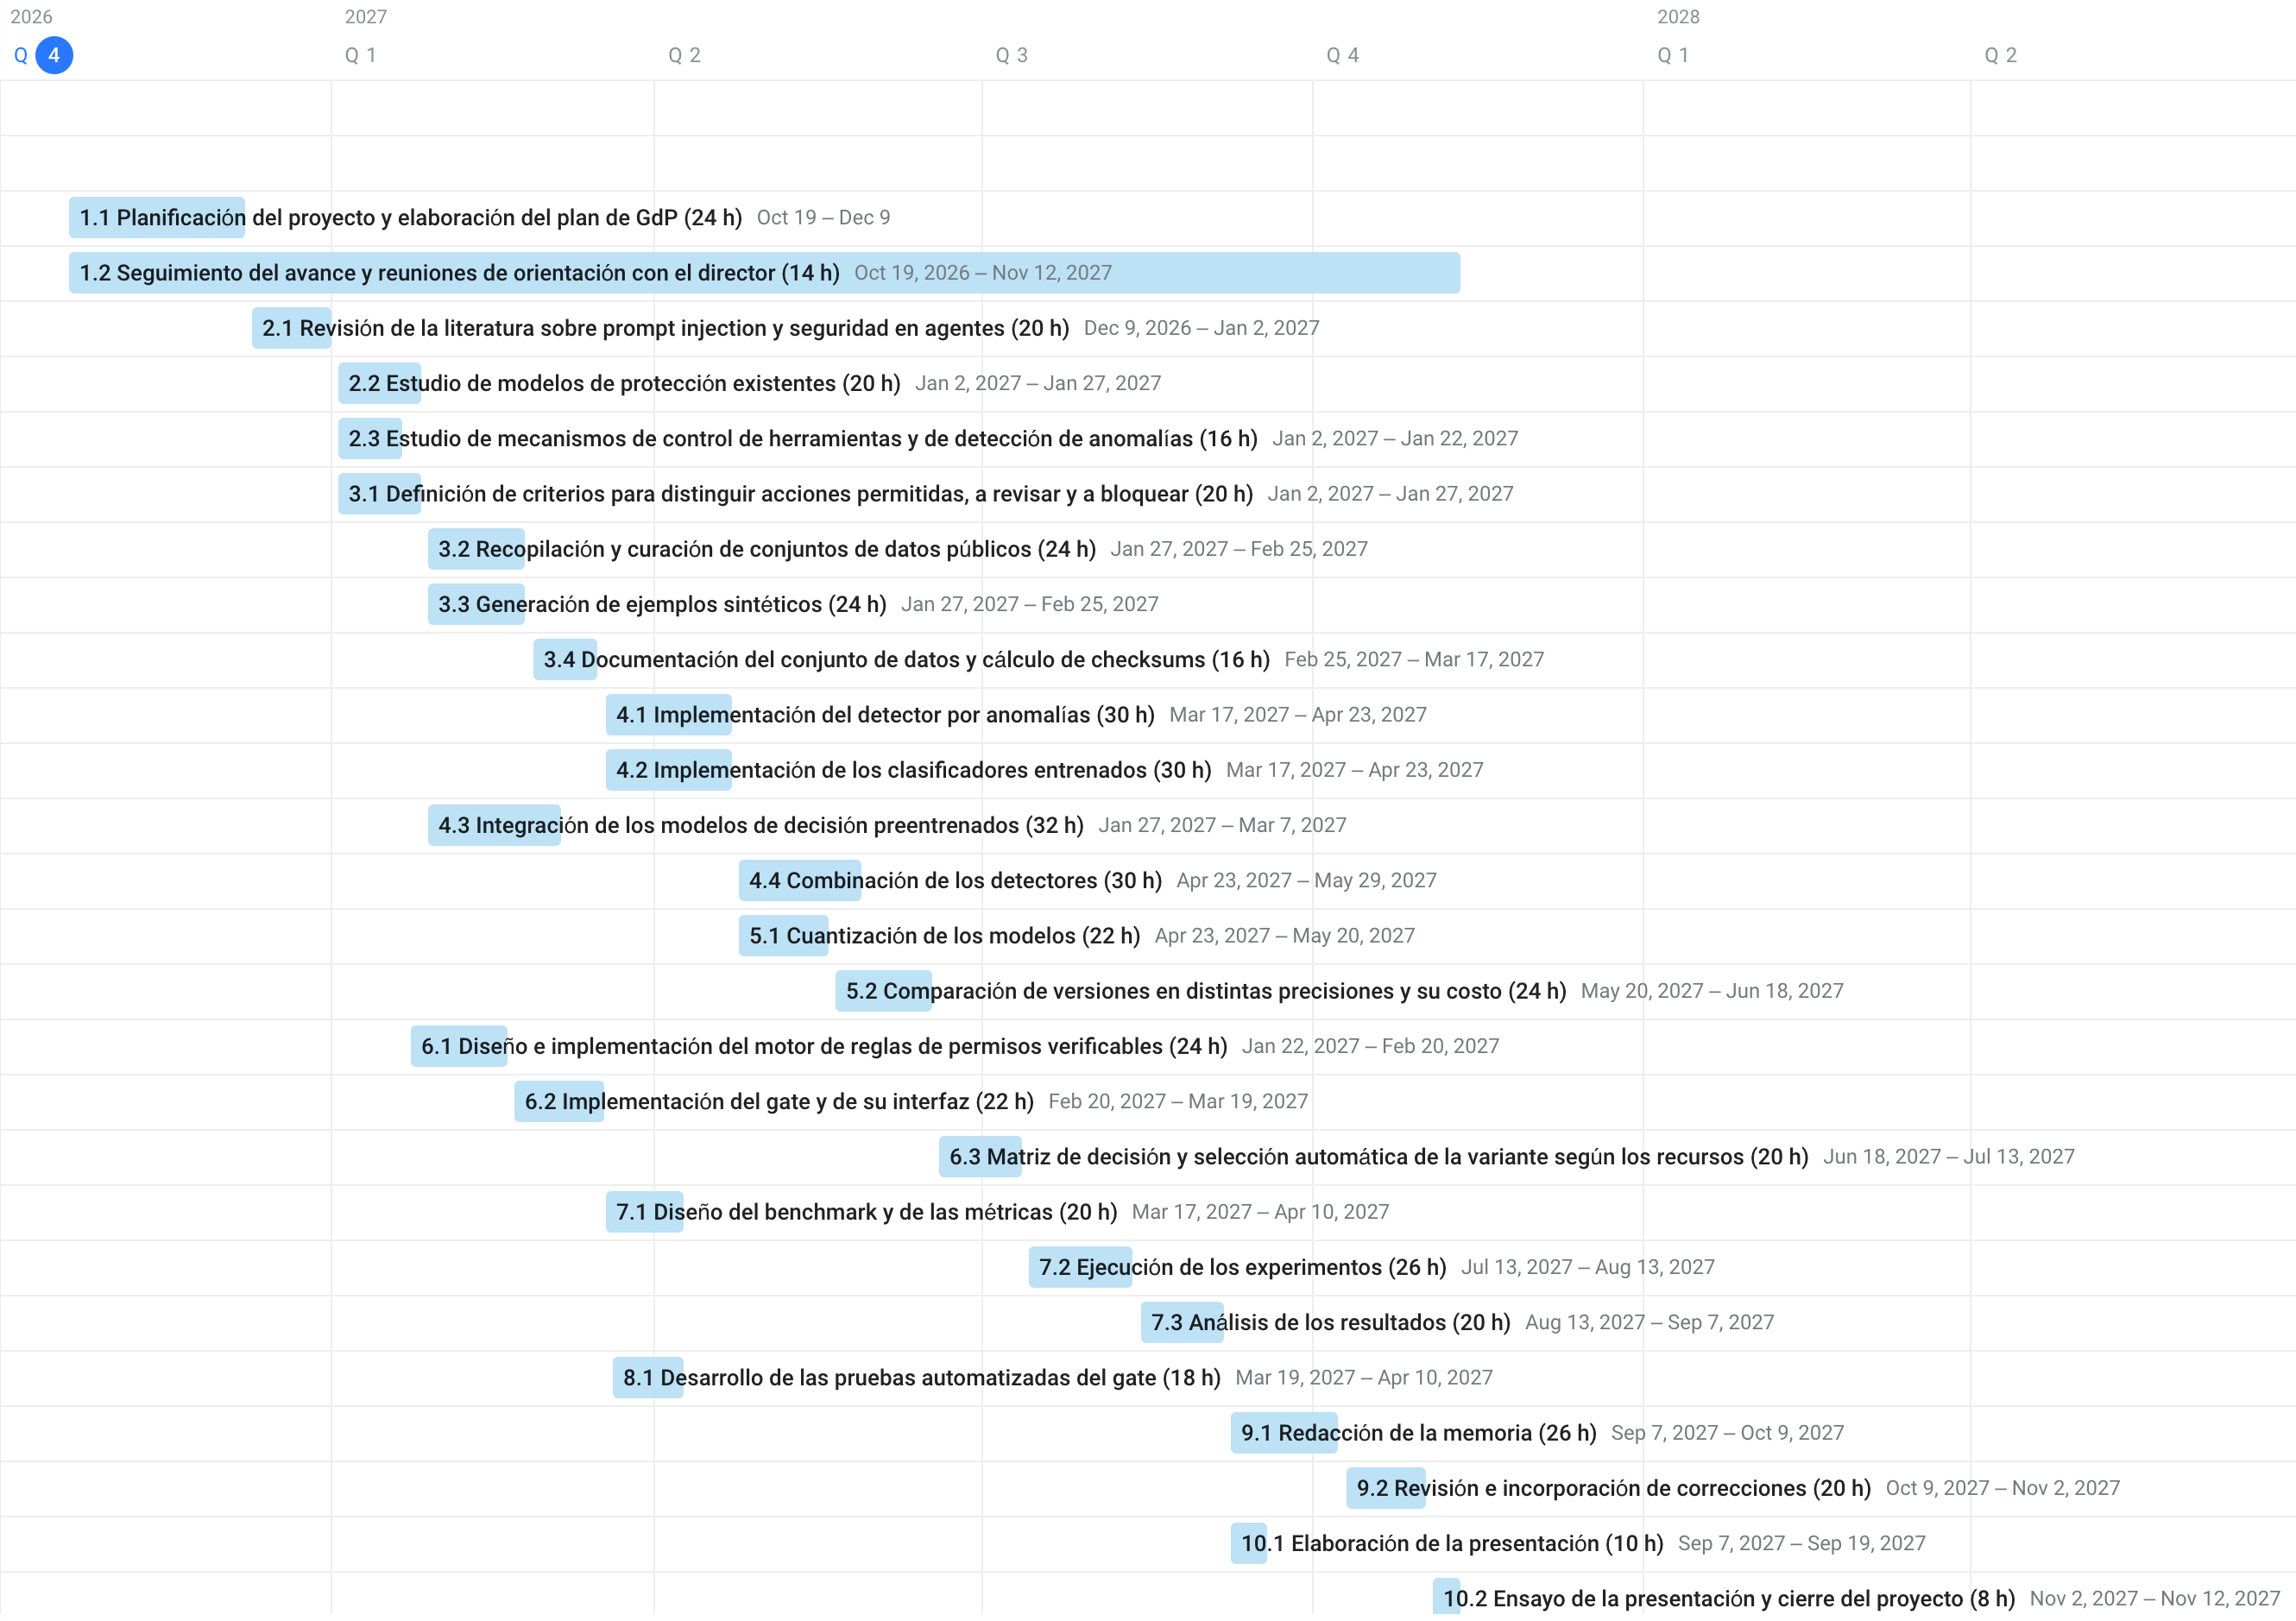
\includegraphics[height=.85\textheight]{./Figuras/Gantt-2.png}
\caption{Ejemplo de diagrama de Gantt (apaisado).} %Modificar este título acorde.
\label{fig:diagGantt}
\end{figure}

\end{landscape}

\end{consigna}


\section{12. Presupuesto detallado del proyecto}
\label{sec:presupuesto}

El presupuesto se expresa en dólares estadounidenses (USD). Dado el período de ejecución (desde octubre de 2026 hasta la defensa prevista en noviembre de 2027), se adopta el USD como moneda de referencia para evitar la distorsión que la inflación introduciría sobre valores expresados en pesos argentinos (ARS).

Al tratarse de un Trabajo Final académico e individual, el mayor componente del costo corresponde a la mano de obra de la responsable. Aunque no implica un desembolso monetario efectivo, se valoriza como costo de oportunidad a un valor hora de mercado de referencia para un perfil semi-senior de IA y datos en Argentina (USD~15/h), por lo que las 600~h estimadas constituyen el principal costo directo.

Los conjuntos de datos públicos, los modelos abiertos y el software utilizado son de uso gratuito, por lo que su costo directo es nulo; se incluyen de todos modos en la tabla para dejar constancia. El cómputo con GPU se cubre mediante una suscripción a Google Colab Pro durante los meses de experimentación. Entre los costos indirectos se consideran la amortización del equipo de cómputo personal, la energía eléctrica y la conexión a internet, imputados de forma proporcional al uso del proyecto.

Los supuestos de cálculo son:
\begin{itemize}
	\item Valor hora de la responsable: USD~15/h (costo de oportunidad, ajustable).
	\item Google Colab Pro: USD~12 por mes durante 5 meses de experimentación (desarrollo de los detectores, optimización y evaluación).
	\item Amortización del equipo: notebook de USD~1.200, vida útil de 48 meses, con 13 meses de uso imputados al proyecto.
	\item Energía eléctrica e internet: imputación proporcional al uso durante el período de ejecución.
\end{itemize}

El detalle se presenta en la tabla~\ref{tab:presupuesto}.

\begin{table}[htpb]
\centering
\caption{Presupuesto detallado del proyecto (en USD).}
\label{tab:presupuesto}
\begin{tabularx}{\linewidth}{@{}|X|c|r|r|@{}}
\hline
\rowcolor[HTML]{C0C0C0}
\multicolumn{4}{|c|}{\cellcolor[HTML]{C0C0C0}COSTOS DIRECTOS} \\ \hline
\rowcolor[HTML]{C0C0C0}
Descripción &
  \multicolumn{1}{c|}{\cellcolor[HTML]{C0C0C0}Cantidad} &
  \multicolumn{1}{c|}{\cellcolor[HTML]{C0C0C0}Valor unit.\ (USD)} &
  \multicolumn{1}{c|}{\cellcolor[HTML]{C0C0C0}Valor total (USD)} \\ \hline
Mano de obra: gestión y organización del proyecto & 40 h & 15 & 600 \\ \hline
Mano de obra: relevamiento y estado del arte & 60 h & 15 & 900 \\ \hline
Mano de obra: conjunto de datos & 90 h & 15 & 1.350 \\ \hline
Mano de obra: desarrollo de los detectores & 130 h & 15 & 1.950 \\ \hline
Mano de obra: optimización y cuantización & 50 h & 15 & 750 \\ \hline
Mano de obra: intermediario (\textit{gate}) e integración & 70 h & 15 & 1.050 \\ \hline
Mano de obra: evaluación y banco de pruebas & 70 h & 15 & 1.050 \\ \hline
Mano de obra: pruebas automatizadas & 20 h & 15 & 300 \\ \hline
Mano de obra: memoria del Trabajo Final & 50 h & 15 & 750 \\ \hline
Mano de obra: presentación y cierre & 20 h & 15 & 300 \\ \hline
Suscripción a Google Colab Pro & 5 meses & 12 & 60 \\ \hline
Conjuntos de datos públicos & --- & 0 & 0 \\ \hline
Modelos abiertos y software de código abierto & --- & 0 & 0 \\ \hline
\multicolumn{3}{|r|}{SUBTOTAL COSTOS DIRECTOS} &
  \multicolumn{1}{r|}{9.060} \\ \hline
\rowcolor[HTML]{C0C0C0}
\multicolumn{4}{|c|}{\cellcolor[HTML]{C0C0C0}COSTOS INDIRECTOS} \\ \hline
\rowcolor[HTML]{C0C0C0}
Descripción &
  \multicolumn{1}{c|}{\cellcolor[HTML]{C0C0C0}Cantidad} &
  \multicolumn{1}{c|}{\cellcolor[HTML]{C0C0C0}Valor unit.\ (USD)} &
  \multicolumn{1}{c|}{\cellcolor[HTML]{C0C0C0}Valor total (USD)} \\ \hline
Amortización del equipo de cómputo (notebook personal) & 13 meses & 25 & 325 \\ \hline
Energía eléctrica (proporcional) & 13 meses & --- & 45 \\ \hline
Conexión a internet (proporcional) & 13 meses & --- & 60 \\ \hline
\multicolumn{3}{|r|}{SUBTOTAL COSTOS INDIRECTOS} &
  \multicolumn{1}{r|}{430} \\ \hline
\rowcolor[HTML]{C0C0C0}
\multicolumn{3}{|r|}{\cellcolor[HTML]{C0C0C0}TOTAL} &
  \multicolumn{1}{r|}{\cellcolor[HTML]{C0C0C0}9.490} \\ \hline
\end{tabularx}%
\end{table}


\section{13. Gestión de riesgos}
\label{sec:riesgos}

\begin{consigna}{red}
a) Identificación de los riesgos (al menos cinco) y estimación de sus consecuencias:
 
Riesgo 1: detallar el riesgo (riesgo es algo que si ocurre altera los planes previstos de forma negativa)
\begin{itemize}
	\item Severidad (S): mientras más severo, más alto es el número (usar números del 1 al 10).\\
	Justificar el motivo por el cual se asigna determinado número de severidad (S).
	\item Probabilidad de ocurrencia (O): mientras más probable, más alto es el número (usar del 1 al 10).\\
	Justificar el motivo por el cual se asigna determinado número de (O). 
\end{itemize}   

Riesgo 2:
\begin{itemize}
	\item Severidad (S): X.\\
	Justificación...
	\item Ocurrencia (O): Y.\\
	Justificación...
\end{itemize}

Riesgo 3:
\begin{itemize}
	\item Severidad (S):  X.\\
	Justificación...
	\item Ocurrencia (O): Y.\\
	Justificación...
\end{itemize}


b) Tabla de gestión de riesgos:      (El RPN se calcula como RPN=SxO)

\begin{table}[htpb]
\centering
\begin{tabularx}{\linewidth}{@{}|X|c|c|c|c|c|c|@{}}
\hline
\rowcolor[HTML]{C0C0C0} 
Riesgo & S & O & RPN & S* & O* & RPN* \\ \hline
       &   &   &     &    &    &      \\ \hline
       &   &   &     &    &    &      \\ \hline
       &   &   &     &    &    &      \\ \hline
       &   &   &     &    &    &      \\ \hline
       &   &   &     &    &    &      \\ \hline
\end{tabularx}%
\end{table}

Criterio adoptado: 

Se tomarán medidas de mitigación en los riesgos cuyos números de RPN sean mayores a...

Nota: los valores marcados con (*) en la tabla corresponden luego de haber aplicado la mitigación.

c) Plan de mitigación de los riesgos que originalmente excedían el RPN máximo establecido:
 
Riesgo 1: plan de mitigación (si por el RPN fuera necesario elaborar un plan de mitigación).
  Nueva asignación de S y O, con su respectiva justificación:
  \begin{itemize}
	\item Severidad (S*): mientras más severo, más alto es el número (usar números del 1 al 10).
          Justificar el motivo por el cual se asigna determinado número de severidad (S).
	\item Probabilidad de ocurrencia (O*): mientras más probable, más alto es el número (usar del 1 al 10).
          Justificar el motivo por el cual se asigna determinado número de (O).
	\end{itemize}

Riesgo 2: plan de mitigación (si por el RPN fuera necesario elaborar un plan de mitigación).
 
Riesgo 3: plan de mitigación (si por el RPN fuera necesario elaborar un plan de mitigación).

\end{consigna}


\section{14. Gestión de la calidad}
\label{sec:calidad}

\begin{consigna}{red}
Elija al menos diez requerimientos que a su criterio sean los más importantes/críticos/que aportan más valor y para cada uno de ellos indique las acciones de verificación y validación que permitan asegurar su cumplimiento.

\begin{itemize} 
\item Req \#1: copiar acá el requerimiento con su correspondiente número.

\begin{itemize}
	\item Verificación para confirmar si se cumplió con lo requerido antes de mostrar el sistema al cliente. Detallar.
	\item Validación con el cliente para confirmar que está de acuerdo en que se cumplió con lo requerido. Detallar. 
\end{itemize}

\end{itemize}

Tener en cuenta que en este contexto se pueden mencionar simulaciones, cálculos, revisión de hojas de datos, consulta con expertos, mediciones, etc.  

Las acciones de verificación suelen considerar al entregable como ``caja blanca'', es decir se conoce en profundidad su funcionamiento interno.  

En cambio, las acciones de validación suelen considerar al entregable como ``caja negra'', es decir, que no se conocen los detalles de su funcionamiento interno.

\end{consigna}

\section{15. Procesos de cierre}    
\label{sec:cierre}

\begin{consigna}{red}
Establecer las pautas de trabajo para realizar una reunión final de evaluación del proyecto, tal que contemple las siguientes actividades:

\begin{itemize}
	\item Pautas de trabajo que se seguirán para analizar si se respetó el Plan de Proyecto original:\\
	 - Indicar quién se ocupará de hacer esto y cuál será el procedimiento a aplicar. 
	\item Identificación de las técnicas y procedimientos útiles e inútiles que se emplearon, los problemas que surgieron y cómo se solucionaron:\\
	 - Indicar quién se ocupará de hacer esto y cuál será el procedimiento para dejar registro.
	\item Indicar quién organizará el acto de agradecimiento a todos los interesados, y en especial al equipo de trabajo y colaboradores:\\
	  - Indicar esto y quién financiará los gastos correspondientes.
\end{itemize}

\end{consigna}

\end{document}